\section{Goldberg And Rao 1998}
\label{GRSection}
The algorithm by A. V. Goldberg and S. Rao, \cite{Goldberg1998}, is a maximum flow algorithm built on the blocking flow paradigm. The main idea is to use a binary length
function on the edges. This means that the edges can have either have 0 or 1 in length as opposed to other algorithms, where they always have length 1. Edges with
large capacity is assigned this new 0 length. The idea is to saturate these large edges earlier by including them in an earlier layer graph. 

Assigning zero length edges might lead to a cycle of zero-length edges. This is an issue, as our blocking flow algorithm only works on DAGs. 
To fix this we contract all the zero-length cycles into super-nodes and run the algorithm on the graph of these instead.
When the blocking flow algorithm is done we route the flow internally in each super-node. This might lead to a problem if 
the flow found is too big to be routed. We therefore decrease the found flow to something we are guaranteed to be able to route before the actual routing is done.

The algorithm keeps a value $F$ as an upper-bound on how much flow that can still be sent from the source to the target.
This means that when $F$ is zero the algorithm is done and have found a maximum flow. Every iteration of the algorithm we
calculate a new value for $F$, but we only update $F$ if the value is less than or equal to $F/2$.

The maximum flow algorithm has a running time of 
$$O\left(\left(\min{n^{\frac{2}{3}},m^{\frac{1}{2}}}\right)m\log{\frac{n^2}{m}}\log{U}\right)$$

The Goldberg Rao Maximum Flow algorithm is described in broads terms with pseudocode in Algorithm~\ref{GRAlg}
\begin{algorithm}
\caption{Goldberg Rao Maximum Flow Algorithm}\label{GRAlg}
\begin{algorithmic}[1]
\Statex
\Procedure{MaxFlow}{$V,E,s,t$}
	\While{$F > 0$}
		\State Update all the distance labels based on the residual edge capacities
		\State Find all the strongly connected components, formed by zero length edges.
		\State Contract all these components into super-nodes
		\State Find the blocking flow
		\If{The blocking flow is too great to be routed within the SCCs}
			\State Adjust the flow.
		\EndIf
		\State Route the flow in the SCCs, then add the flow to the graph.
		\State Update $F$ if necessary.
	\EndWhile
	\State \Return $e(t)$
\EndProcedure
\end{algorithmic}
\end{algorithm}
In the Sections~\ref{GR-Parts-Start} to~\ref{GR-Parts-end} we describe how the different steps of the algorithm are achieved. 
Some of these steps requires algorithms described in other papers, each of these algorithms have their own Section at the end of 
Section~\ref{GRSection}. Before that we analyse the correctness and running time in Section~\ref{GR-Cor} and~\ref{GR-RT}, respectively.
Section~\ref{GR-IM} describes the modifications we have done in the implementation of the maximum flow algorithm.

In the following sections we will use the following short-hand notation $$\Lambda = \min{\{n^{\frac{2}{3}},m^{\frac{1}{2}}\}}$$
We will also use SCC to denote a strongly connected component.

\subsection{Updating The Distance Labels} \label{GR-Parts-Start}
Every edge is assigned a binary length to it. Based on these lengths each node $v$ is giving a \emph{distance labelling} $d(v)$. The distance labelling
must have the following properties: $d(t) = 0$ and $d(v) \leq d(w) + l(v,w)$ for all edges with positive residual capacity.
$l(v,w)$ is a length function $l: E \to \{0,1\}$. If the length of an edge $(v,w)$ satisfy the distance labelling equation with equality we call the edge \emph{admissible}.
We call the graph where the only edges are the admissible edges the \emph{admissible graph}. the admissible graph is a layer graph.

We base the length function on an value called $\Delta$ and use the following binary length function:

$$ l(v,w) =
  \begin{cases}
   0 & \text{if } r(v,w) \geq 2\Delta \\
   1       & \text{otherwise}
  \end{cases}$$\\
So that edges with large capacities have zero-length. We want the distance from the source to the target to increase when we augment with a blocking flow.
Therefore special consideration has to be given to the place where a zero-length edge $(v,w)$ exist in one direction, and its linked-edge $(w,v)$, 
has a capacity, close to $2\Delta$. When augmenting flow along $(v,w)$ this could then lead to $(w,v)$ becoming a
zero-length edge. Which could case the labels of $v$ and $w$ to stay the same and the distance between $s$ and $t$ to remain the same. To fix this we call edges $(v,w)$ that satisfies
the following three constraints \emph{special}:
\begin{enumerate}
	\item $\Delta \leq r(v,w) \leq 2\Delta$
	\item $d(v) = d(w)$
	\item $r(w,v) \geq 2\Delta$, which would mean $(w,v)$ is a zero edge in the previous definition
\end{enumerate}
Based on the special edge we use the following length function instead:
$$ \bar{l}(v,w) =
  \begin{cases}
   0 & \text{if } r(v,w) \geq 2\Delta \text{ or } (v,w) \text{ is special}\\
   1       & \text{otherwise}
  \end{cases}$$\\

The distance labels are actually the same regardless whether you use $l$ or $\bar{l}$. 
The change is that the special edges now also can be used to send flow over, and that any nodes $v$ and $w$ with a special edge linking them has to be in a zero-length cycle together, so they are contracted.
The reason why we choose that the residual capacity of a special edge should be in the range $[\Delta;2\Delta]$ is that we will later bound
the value of the augmenting flow to be at most $\Delta$, see Section~\ref{GR-RT}.

When we update the distance labels we do it by using a modified BFS.
We have a value $i$ for the current distance label we are assigning to nodes. We initialize $i$ to 0.
We keep two queues. One with nodes we should assign $i$ to called 'the current-queue' and one with nodes we should assign $i+1$ to called 'the next-queue'. 
Whenever we process a node $v$, we look at all its incoming edges. If the edge $(w,v)$ has positive residual capacity we calculate the length of the edge
using $\bar{\ell}$. If the length of $(w,v)$ is zero we add node $w$ to the current-queue, otherwise we add it to the next-queue. Whenever a node has been
fully processed we get the next node to process from the current-queue. When the current-queue is empty we increase $i$ by one and
use the next-queue as the the current-queue and vice versa.  We start this method by processing the target node, and are done when both queues are empty.

To prevent us from processing the same node several times we reset the distance label of each node in the graph to $\infty$ before we process them. 
Then we can recognize whether a node has been processed by looking at its label.

The time to reset the labels are $O(n)$
As each edge is only considered once in this modified BFS the running time is $O(m)$. The total time to update the labels are therefore $O(m+n) = O(m)$.

\subsection{Finding All The Strongly-Connected-Components}
To find all SCCs composed of only zero-length edges we use a slightly modified version of an algorithm made by R. E. Tarjan, \cite{Tarjan1972}.
The running time of the algorithm is $O(m)$. For further details on this algorithm see Section~\ref{GR-SCC}. 
The returned value of the algorithm is a list of sub-lists. Each sub-list contains a number of nodes which form a SCC.

\subsection{Contracting The Strongly Connected Components}
When we run the blocking flow algorithm each super-node consist of a bunch of sub-nodes. The edge-list of the super-node is made by
having an iterator run through the edge-lists of the sub-nodes. To prevent any overhead to occur we give each super-node a list of all the sub-nodes
it consists of. We also runs through all the sub-nodes and gives them a link to the super-node representing them. In this manner we can work
with the super-nodes with only $O(1)$ amount of overhead.

There exists at most $n$ super-nodes. The initialization of each super-nodes takes $O(1)$ time, when not counting the time to make the lists of sub-nodes.
The total time to make these sub-lists sums to $O(n)$. The last thing we do is to set up the pointer from the sub-nodes, this also takes $O(n)$ time.
Combine these running time and the cost of contraction, which is the cost to set up the super-nodes, is $O(n)$.

\subsection{Finding The Blocking Flow}
To find the blocking flow in the graph consisting of super-nodes we use an algorithm by  A. V. Goldberg and R. E. Tarjan, \cite{GoldbergTarjan1990}. 
Further details on the algorithm can be seen in Section~\ref{GR-BF}. 
The blocking flow algorithm runs in $$O(m\log{\frac{n^2}{m}})$$
We have modified the blocking flow algorithm slightly. The analysis of how this affect the running time of the maximum flow algorithm
can be found in Section~\ref{GR-IM}

The result of the algorithm is a flow, that could be used to augment the current flow to get a blocking flow in the admissible graph.

\subsection{Adjusting The Flow}
If the flow $f$ found in the previous Section has a value greater than $\Delta$ then we have no guarantee that we can route it internally in the super-nodes.
We therefore decrease $f$ in the following manner.

Set $U = f - \Delta$. Place $U$ units of excess at the target node. Process each node in a reverse-topological order. When 
processing a node, decrease the flow on incoming edges until the excess is zero.

Since each edge is only considered once this has a running time of $O(m)$.

\subsection{Routing the flow}
To route the flow internally in each SCC we use an algorithm by B. Haeupler and R. E. Tarjan, \cite{Haeupler2007}. For more details see Section 
\ref{GR-RF}. The motivation for the algorithm was that the authors observed you could get a small constant factor decrease in the theoretical
running time of the A. V. Goldberg And S. Rao maximum flow algorithm by doing it.
Using the new algorithm saves us a $\Delta$ on the length-functions. The original article had $l(v,w)$ being zero only if the residual
capacity was higher than $3\Delta$. The effect of the change is included in the running time Section~\ref{GR-RT}

The running time of this algorithm is $O(m)$.

When the routing algorithms has been run, a flow $f$ of most $\Delta$ has been found and routed. 
We therefore augment the flow in graph with $f$.
This means running through all edges, adding the new flow and updating the residual capacity of each edge and its linked edge.
This takes $O(m)$ time.

\subsection{Updating $F$} \label{GR-Parts-end}
$F$ represents an upper bound on the flow that can still be send from the source to the target. 
This value must be lower or equal to the value of every $S,T$-cut. This is because it is the dual problem. 
This means that if we could saturate a $S,T$-cut then it would be the min-cut, if the cut could not be saturated then it is because another cut with a
smaller capacity have been saturated. This smaller cut has to be the min-cut. Therefore the $S,T$ cut had a capacity greater than the min-cut.

To bound $F$ from above we therefore find a series of cuts. A \emph{canonical cut} is a cut $S_k,T_k$ where 
$S_k = \{v \in V \mid d(v) \geq k\}, T_k = V \setminus S_k$.

To calculate the canonical cuts we initialize an array with $d(s)$ entries. We iterate over all edges. If the nodes of an edge $(v,w)$
have distances $d(v) > d(w)$ then we add the residual capacity of the edge to entry $d(v)$ in the array. When done
we find the minimum among the cuts. If this value is less than $F/2$ we update $F$ to this value.

We use $O(1)$ time per edge. We initialize an array of at most $n$ entries, and scan it once. This leads to a running time of
$O(m+n) = O(m)$.

We have now described all the different pieces of the algorithm. The next sections will show the correctness of the algorithm and
analyse the running time.

\subsection{Correctness} \label{GR-Cor}
We keep augmenting the flow in the graph by flow found by the blocking flow algorithm. Assuming the blocking flow is valid
and the routing of the flow is also valid the flow stays valid throughout the run of the maximum flow algorithm. 

We do sometimes change the blocking a little before we route it. This happens if the amount sent in the blocking flow algorithm is too large.
When we decrease it we keep making sure that the excess of all nodes, besides the source and target node, stay zero. Therefore the 
flow must still be a valid flow after the decrease.

$F$ represent the maximum amount of flow we can still send from the source to the target, and we keep augmenting until $F$ is zero. 
This must mean that the flow at this point in time is a maximum flow, as no augmenting path exists.
	
\subsection{Running Time} \label{GR-RT}
We need to have an initial value for $F$. We look at an initial $S,T$-cut, where the set $S$ only consist of the source node and $T$ then the rest.
Only the edges from the source crosses the cut. That is at most $n$ edges. Each edge has at most $U$ capacity. Therefore we initialize $F$ to
$nU$. We define a phase to be a number of iterations until $F$ is updated. This means $F$ is at least halved every new time a phase starts. 
Which means we have at most $\log{nU}$ phases.
	
We will now bound how much work is done in each iteration. We have already described all the operations
done each iteration, and they all, except the blocking flow algorithm, have a running time of $O(m)$.
The running time of the blocking flow is $O(m\log{\frac{n^2}{m}})$. 
Summing up all the contributions therefore gives a running time for each iteration of $O(m\log{\frac{n^2}{m}})$.

We will look at how many iterations can be done each phase. We bound the number of iterations done where the augmenting flow is not a blocking flow. 
We used $\Delta$ to bound the value of each augmenting non-blocking flow.
If we want to get the wanted total running time of $O\left(\Lambda m\log{\frac{n^2}{m}}\log{nU}\right)$, then the number of non-blocking iterations
per phase can be no more than $O(\Lambda)$.
We therefore set $\Delta$ equal to $\frac{F}{\Lambda}$. This means that after $O(\Lambda)$ non-blocking iterations $F$ has to be updated and a new phase
is begun.

To bound the number of blocking iterations in each phase we want an upper bound on the capacity of the minimum canonical cut.

\begin{lemma} \label{GR-MinCut-m}
	Using a binary length-function the capacity of the minimum canonical cut satisfies: 
	$$\text{cap(min-canonical-cut)} \leq \frac{mM}{d(s)}$$
	Where M is the maximum residual capacity of all the edges with length 1.
\end{lemma}
\begin{proof}
	The sum over all edges of their residual capacities has to be less than or equal to $mM$. There has to exist $d(s)$ cuts.
	Therefore the minimum has to satisfy the equation. $\square$
\end{proof}
If the graph is dense, meaning that $m$ is high, a better bound of the minimum canonical cut can be found in the following lemma. We use the same
terminology as in the previous one.
\begin{lemma}\label{GR-MinCut-n}
	$$\text{cap(min-canonical-cut)} \leq \left(\frac{2n}{d(s)}\right)^2 M$$
\end{lemma}
\begin{proof}
	We define $V_k = \{v \in V \mid d(v) = k\}$. We want to show that there exist a $k$ such that both $V_k$ and $V_{k+1}$ contains at most
	$\frac{2n}{d(s)}$ nodes. If this is the case then the total amount of edges is less than or equal to $\left(\frac{2n}{d(s)}\right)^2$, this gives
	a maximum cut value of the stated value in the lemma.
	
	We know that $\sum_{k = 0}^{d(s)}{|V_k|} = n$. Using the pigeon hole principle that means that at least $\lceil d(s)/2\rceil + 1$ of the sets $V_k$ has
	at most $\frac{2n}{d(s)}$ nodes. Therefore there has to exist two consecutive sets with at most this number of nodes, giving us the lemma. $\square$
\end{proof}

Only edges with length 1 is counted in the canonical cuts. Therefore $M$ has to be lower or equal to $2\Delta$.

\begin{lemma}
	If we assume that the distance between the source and the target node increases after a blocking flow. Then there is at most $O(\Lambda)$ blocking
	iterations per phase.
\end{lemma}
\begin{proof}
	Suppose $\Lambda$ is $m^{1/2}$. Every blocking flow iteration increase the distance to the source by at least one.
	Then after $4\Lambda$ iterations $d(s)$ has to be greater than or equal to $4m^{1/2}$. Combined with Lemma~\ref{GR-MinCut-m} this gives the following equations:
	$$\text{min-canonical-cut} \leq \frac{mM}{d(s)} \leq \frac{m2}{d(s)} \Delta \leq \frac{m2}{4m^{1/2}}\frac{F}{m^{1/2}} = \frac{F}{2}$$
	This means that after at most $4\Lambda$ iterations the phase ends, regardless of how many non-blocking iterations have been made.
	If we used the original length-function the number of iteration would have been $6\Lambda$ instead of $4\Lambda$. 
	
	A similar calculation can me made if $\Lambda$ is $n^{2/3}$. Here $4\Lambda$ iterations are needed. Combined with Lemma~\ref{GR-MinCut-n} this is:
	$$\text{min-canonical-cut} \leq \left(\frac{2n}{d(s)}\right)^2 M \leq \frac{8n^2}{d(s)} \Delta \leq \frac{8n^2}{4^2n^{4/3}} \frac{F}{n^{2/3}} = \frac{F}{2}$$
	$\square$
\end{proof}
So we have $O(\Lambda)$ iterations between phases. Each iteration takes $O(m\log{\frac{n^2}{m}})$ time. Combined with the fact that the number of
phases is $O(\log{nU})$ This gives a total running time of $O(\Lambda m\log{\frac{n^2}{m}} \log{nU})$. 

The next Theorem reduces the running time to the one we want.
\begin{theorem}
	The running time of the maximum flow algorithm is $$O(\Lambda m\log{\frac{n^2}{m}} \log{U})$$. Assuming a blocking flow increases the distance from $s$ to $t$
\end{theorem}
\begin{proof}
	We will look at the work done when $\Delta$ is in three different value ranges.
	
	$\Delta = 1$. If $\Delta$ is equal to 1 the algorithm finishes after $\Lambda$ iterations. If $\Delta$ is 1 then that means that $F$ is less than or equal to
	$\Lambda$. Each iteration augments the flow with 1. Combining these facts mean that $F$ is an upper bound on the number of iterations.
	
	$\Delta \in ]1:U]$. In this interval there has to be $\log{U}$ phases by the way we have defined $F$ and $\Delta$. The number of phases are equal
	to the number of times we halves $F$. When we halve $F$ we also halve $\Delta$, as $\Delta$ is equal to $\frac{F}{\Lambda}$, $\Lambda$ is constant
	throughout the run of the algorithm. 
	The number of times we can halve $\Delta = U$ before it reaches 0 is $\log{U}$.
	
	$\Delta > U$. In this case the number of iterations are also equal to $\Lambda$. As $\Delta$ is greater than $U$ every edge has to have length 1. It
	also means that every iteration has to be a blocking flow. Therefore after $2\Lambda$ iterations the distance of the source, $d(s)$, has to be greater or
	equal to $2\Lambda$. Then that means that after at most $2\Lambda$ iterations $F \leq \Lambda U$, which implies that $\Delta$ is less than or equal to $U$.
	We can prove the previous statement by using Lemma~\ref{GR-MinCut-m} and~\ref{GR-MinCut-m}:
	If $\Lambda = m^{1/2}$ then:
	$$F \leq \frac{m}{d(s)} M \leq \frac{m}{2m^{1/2}}U < m^{1/2}U = \Lambda U$$
	If $\Lambda = n^{2/3}$ then:
	$$F \leq \frac{4n^2}{d(s)^2}M \leq \frac{4n^2}{4n^{4/3}}U = n^{2/3}U = \Lambda U.$$
	
	The amount of phases done by the algorithm can therefore be reduced to $\log{U}$. The rest of the work is hidden by the O-notation removing the constant
	in front of $\Lambda$. $\square$
\end{proof}

We now to show that the distance from the source to the target is increasing when a blocking flow is used to augment the current flow in the graph.
We denote distance labelling giving based on a length function $l$ $d_l$. We use $l$ for the unmodified version of the distance function and $\bar{l}$ for
the modified one.
\begin{theorem}
	Let $\bar{f}$ be the a flow found in the graph of admissible edges. $f' = f + \bar{f}$ is the flow after the current flow has been augmented with $\bar{f}$.
	Let $l'$ be the length function corresponding to $f'$. Then we want to show the three following statements
	\begin{enumerate}
		\item The distance labelling $d_l$ used to calculate $\bar{f}$ is also a distance labelling with respect to $l'$.
		\item $d_{l'}(s) \geq d_{l}(s)$.
		\item If $\bar{f}$ is a blocking flow then $d_{l'}(s) > d_{l}(s)$.
	\end{enumerate}
\end{theorem}
\begin{proof}
	For the proof, please see \cite[Lemma 4.1]{Goldberg1998}, \cite[Corollary 4.2]{Goldberg1998} and \cite[Theorem 4.3]{Goldberg1998}.
	$\square$
\end{proof}

\subsection{Implementation Modifications} \label{GR-IM}

Since we used a modified version of the blocking flow algorithm with a running time of $$O\left((n^2 + nm)\log{\frac{n^2}{m}}\right)$$ 
Instead of only $O(m\log{\frac{n^2}{m}})$ we get a factor $n$ slowdown throughout each iteration, which also means a factor $n$ slowdown in the
total running time, giving a running time of $$O\left(\left(\min{n^{\frac{2}{3}},m^{\frac{1}{2}}}\right)nm\log{\frac{n^2}{m}}\log{U}\right)$$
for the maximum flow algorithm.

When we decrease the flow found in the blocking flow algorithm, in case it is too large, we do not do it in a reverse topological order. 
We do not do any topological sorting, since our modified version of the blocking flow algorithm does not require it.
We instead keep a queue over the nodes to process. When a node is processed it decreases any incoming flow until its excess is zero. 
We start the process by putting the target in the queue. We define pass $i+1$ over the queue to mean to process all the nodes added in pass $i$.
The first pass, pass zero, is when we add the target to the queue. The flow does not contain any cycles, this means that when we decrease the
flow in each pass, we move it one edge closer to the source. As the maximum length of a path is $n$ this gives at most $n$ passes.
Each node does a constant amount of work on each edge it decreases on. The amount on edges sums to $m$ meaning that the total running time
of this decreasing flow algorithm is $O(nm)$. The original algorithm only took $O(m)$ time. The time does not affect the total running time,
as we have already increased it by $n$ per iteration by using the modified blocking flow algorithm.

It may happen that the source and the target is in the same super-node. In this case the algorithm may fail, so the algorithm does these iteration in a special 
fashion. Since we know that we can send $\Delta$ flow from the source to the target internally in the strongly connected component they are both a part
of, we skip the blocking flow calculation. Instead we just run the routing flow algorithm. we make sure that the source it the root of the trees being
constructed and then we place a demand with value $\Delta$ in the target and route it as usually. This does not affect the running time in any negative way.


\subsection{Tarjan's SCCs Algorithm} \label{GR-SCC}
The algorithm was designed by R. E. Tarjan and published in 1972, \cite{Tarjan1972}.

The algorithm returns a list of sub-lists. Each sub-list consists of nodes which are in the same SCC.

The general idea is that you iterate over unprocessed nodes. When you process a node $v$ you push it on a stack. Then you recursively visit and process all
its friends if they are unprocessed. The friends are all the nodes where $v$ has an outgoing edge with positive residual capacity to.
The recursion is done in a DFS manner.

A node is marked if it is on the stack.

Every node is given an unique index, which is given the first time they are pushed onto the stack. The indexes given start at zero and is increased by one each
time a new one is given,
in this way you can distinguish in which order the nodes were pushed on the stack.
Each node also has a value called the lowlink, which represent the lowest node on the stack which is an friend. It starts out being its own unique index.

When you process a node $v$ and it has chosen a new friend to visit if the friend is on the stack $v$ updates its own lowlink to the minimum of its current lowlink
and the friend's lowlink.

sWhen returning from the recursion on a friend a node similarly updates it lowlink to be the minimum of its current lowlink and the friend's lowlink.

If a node $v$ has run through its entire list of friends it is done. If it has a lowlink value lower than its own index then it is allowed to stay on the 
stack, otherwise it and everything above it on the stack is popped off. 

If $v$ is popped and its lowlink is still equal to its own index, then $v$ has to be part of a strongly connected component with all the elements on top of it. 
This has to be the case as all of them were put on the stack later based on a DFS starting from $v$. 
Since they are still there they have to have a lowlink lower than them selves, but $v$ would have gotten this same value
meaning $v$ has to be the one they all have a lowlink to. Leading to the fact that $v$ can reach them and they can all reach $v$, so they are part
of the same SCC. 

The algorithm creates a new sub-list whenever it encounters a node $w$ that has its lowlink being equal to its own unique index. The sub-list is filled
with $w$ and all the nodes above it.

Each node is only processed once, where its entire edge-list is read through once. This sums up to $O(n+m)$ over all nodes.

\subsubsection{Implementation modifications}
The maximum flow algorithm only contracts strongly connected components that are linked by zero-length edges. Therefore the algorithm to find 
SCCs has been changed to only visit nodes connected with edges of zero-length.

As we ran the algorithm on large graphs we ran into an issue with the recursion. The stack-frames for each recursion simply takes up to much space.
If we have a massive SCC component it is all on the stack and a lot of recursions have been done, leading to all the memory being spent and
the algorithm crashing. Therefore we transformed the algorithm to avoid recursion. This
allowed us to run on larger instances.


\subsection{Goldberg Tarjan Blocking Flow Algorithm} \label{GR-BF}
To find the blocking flow in a layered graph the maximum flow algorithm uses the blocking flow algorithm made by A. V. Goldberg and R. E. Tarjan \cite{GoldbergTarjan1990}.
The blocking flow algorithm has a running time of $$O(m\log{\frac{n^2}{m}})$$
The general concept of the blocking flow algorithm is in the paper, though the proof of correctness and the running time is left to the reader. 
The proofs are left out in the original paper because there is another algorithm in the paper that has an analysis similar to the blocking flow algorithm.
We found an error in the theory, so we have made an addition to fix the error. It can be seen in Section~\ref{gr-fixing}

The algorithm has a lot in common with a maximum flow push relabel algorithm. It also works by manipulating a pre-flow.
The blocking flow algorithm only works on a DAG.

Every node in the graph is either in a \emph{blocked} state or in a \emph{unblocked} state. If a node is blocked it means that the node can not be pushed to. At
the beginning of the algorithm all nodes are unblocked and they can only go from being unblocked to being blocked.

The algorithm works by first saturating edges leaving the source. Afterwards it pushes the excess around. If at some point a node
can not push the flow further it blocks itself and starts pulling the flow backwards instead. When a node pulls it moves the excess back towards where it came from
by decreasing the flow on incoming edges with flow on. The algorithm terminates when the excess of all nodes, besides the source and target, is zero.

\begin{algorithm}
\caption{Blocking flow Push, Pull and Block procedures}\label{BFPushPullBlock}
\begin{algorithmic}[1]
\Statex
\Procedure{Push}{ Edge $(v,w)$ }
	\State Transfer $\delta = \min{(e(v), r(v,w))}$ units of flow by updating the edges, $(v,w)$ and $(w,v)$, and the excess, $e(v)$ and $e(w)$.
\EndProcedure
\Statex
\Procedure{Pull}{$ Edge (v,w)$}
	\State Subtract $\delta = \min{(e(w), f(v,w))}$ units of flow on $(v,w)$ by updating the edges, $(v,w)$ and $(w,v)$, and the excess, $e(v)$ and $e(w)$.
\EndProcedure
\Statex
\Require {$\forall(v,w) \in E: r(v,w) = 0$ or $w.blocked$}
\Procedure{Block}{$v$}
	\State $v.blocked \gets true$
\EndProcedure
\end{algorithmic}
\end{algorithm}

The three main operations can be seen in Algorithm~\ref{BFPushPullBlock}.

All three operations only apply to \emph{active} nodes. A node is active if it has positive excess.

The push method moves excess from node $v$ to $w$ by adding flow on the edge $(v,w)$. The amount of excess moved is the minimum of the excess of $v$ and the
residual capacity of edge $(v,w)$, in this way the excess never goes negative, and the capacity constraint is not violated. 
When doing a push the receiving node $w$ can not be blocked.

The block operation blocks a node if the algorithm can not do a push operation on any of its outgoing edges. A push can not be done on an edge if either the residual 
capacity is 0 or the receiving node is blocked.

The pull operation works on an edge $(v,w)$ and only applies if node $w$ is blocked. It pulls flow sent to $w$ from $v$ back by subtracting
the minimum of the excess in $w$ and the flow on $(v,w)$ from the flow on $(v,w)$. The pull operation only makes sense to apply to an edge with flow on it.

To know which edge to do a pull or push operation on each node has an edge pointer called the \emph{current-edge}. The current-edge is initially
set to the first edge in a node's edge list. If neither a pull nor push operation applies to the current-edge of a node, the next edge in the node's edge list
is set as the current-edge. If the current-edge was the last edge of the node, then the current-edge resets to the first edge and a block operation is done.

The algorithm uses the dynamic-trees data structure, see Section~\ref{Dynamic Trees} for a description. Each node in the graph also has a node in the dynamic
tree representing it, all nodes in the dynamic tree start out not linked. The idea is to link two nodes in the dynamic tree if the edge between them can either 
be pulled or pushed upon later. This way entire paths in the graph can be saved in the dynamic tree. The value on each node in the dynamic tree shows how much flow 
can either be pulled or pushed on the edge to the parent. 
In the case of it being linked as part of a push operation we call it a \emph{push edge} and the value saved is the residual capacity of the edge. 
Otherwise it is a \emph{pull edge} and the value is instead the flow on the edge. 
This means that flow can be pulled and pushed along an entire path simple by doing an AddCost operation on the dynamic tree.
A path of length $k$ takes amortized $O(\log{k})$ to do an operation on, but in this case doing the equal amount of push and pull operations would take $O(k)$ time,
so adding the data structure saves time.

The addition of the dynamic trees gives some changes when pushing and pulling. Now in addition to doing a push/pull operation the algorithm also does a send operation.
If after a send operation an edge $(v,w)$ has enough flow/residual-capacity to do a pull/push the node $v$ is linked to $w$ 
in the dynamic tree, and the edge $(v,w)$ is saved there as well. 
This is where we can distinguish whether the edge is a push or pull edge, if it is saved as part of a Link operation done after a push operation it is a push edge, 
otherwise it is a pull-edge.
The linking is only done if the combined size of the dynamic trees containing $v$ and $w$ are lower than a
constant $k$, $v$ is a root and $v$ and $w$ are not already in the same tree. All this logic can be seen in pseudocode in Algorithm~\ref{BFPushPullRelabelDischarge},
in the Tree-PushPullBlock method. The constant $k$ should always be equal or larger than two to make sure that the dynamic trees are used.

Something to note is that the values in the tree are not synchronized with the values on the edges. The values meaning the residual capacity or the flow.
The issue is that keeping the values completely synchronized would mean that when doing an AddCost operation all the edges should be updated. This
means the cost becomes $O(k)$ instead of amortized $O(\log{k})$ for a path of length $k$, destroying the entire reason to use dynamic trees.
To make sure this mismatch of values does not become a problem an invariant is introduced; saying that all nodes that are active has to be a root in the dynamic
tree. A root does not have a linked edge to push/pull on in the dynamic tree, so there are no value that has to be synchronized, this also means that the
value of a root does not have any meaning and is generally ignored, only the excess of the root matters.

To keep the invariant any new excess added to a path has to be transferred to the root. It might be that a node $v$ on the path has a too low value to do
this. In this case enough excess is transferred to use all the value on the edge $e$ between $v$ and its parent. Afterwards the edge $e$ is cut and
the algorithm reiterates with the rest of the excess. This keeps going until either all the excess has been moved to roots or the active node
has itself become a root, fulfilling the invariant. When cutting a node in this way the actual value are updated with the value from the tree.
If it is a pull-edge this means setting the flow to 0, if it is a push-edge this instead means setting the residual capacity to 0, which in actuality is setting
the flow of the edge equal to the capacity of the edge. All this combined is called the send method. Algorithm~\ref{BFSend} shows the pseudocode for it.

Whenever a node $v$ is being blocked, flow can not be pushed to it. To prevent the dynamic trees from doing an AddCost operation, corresponding to a push, each 
child of $v$, which has a push edge to $v$, is cut loose. The values are then updated for the edges in the graph based on the edges cut in the tree.

\begin{algorithm}
\caption{Blocking Flow Send procedure}\label{BFSend}
\begin{algorithmic}[1]
\Statex
\Statex
\Require $v$ is active
\Procedure{Send}{$v$}
	\While{$\Call{GetRoot}{$v$} \neq v$ and $e(v) > 0$}
		\State $\delta \gets \min{(e(v), \Call{FindMinValue}{v}})$
		\State send $\delta$ value of flow  in the tree by calling $\Call{AddCost}{v,-\delta}$
		\While{\Call{FindMinValue}{$v$} = 0}
			\State $u \gets \Call{FindMin}{$v$} $
			\State $e \gets (u,parent(u))$
			\If{$e$ is an push-edge}
				\State $f(e) = c(e)$
			\Else
				\State $f(e) = 0$
			\EndIf
			\State $\Call{Cut}{$u$} $
		\EndWhile
	\EndWhile
\EndProcedure
\Statex
\Function{FindMinValue}{$v$}
	\State $minNode \gets \Call{GetMinCostNode}{$v$}$
	\State \Return \Call{GetCost}{$minNode$}
\EndFunction
\end{algorithmic}
\end{algorithm}
The algorithm uses a data structure to keep track of all the active nodes. It is a linked list $L$ of sub-lists. 
The first element of each sub-list is called the \emph{head}. 
The invariant on the data structure is that every head of a sub-list, besides the head of the first sub-list, 
has to be an active node and each active node has to be a head in a sub-list. 
To maintain this invariant the sub-lists need to be split or concatenated when nodes become active or inactive. 

The initial state of $L$ is a single sub-list containing all nodes in the algorithm sorted in topological order. 

When a node becomes active the sub-list containing the node is split right before the node and the new sub-list is added to the $L$ as a
succeeding sub-list of the one it was previously a part of. 

When a node becomes inactive the sub-list containing the node is concatenated to the preceding sub-list, if such a list exist. 

If a node $v$ is blocked it is moved to the front of the entire structure. This is done by deleting $v$ in the list it is a head of and
then adding it as the first element of the first sub-list of $L$. The deletion is done by splitting out $v$ and then removing the sub-list containing 
only it. The addition is done by concatenating $v$ with the rest of the first sub-list.

When doing a split the outcome is two sub-lists $s_1$ and $s_2$. When doing concatenations we concatenate two sub-lists $s_1$ and $s_2$.
If we scanned through the sub-lists to concatenate and split we would use linear time in the size of the smaller sub-list to do so.
To do this faster every sub-list is represented as a Finger tree data structure instead. This data structure can do splits and concatenations in
logarithmic time instead of linear.

The discharge method in the blocking flow algorithm takes the first active head from $L$ and keeps calling the Tree-PushPullBlock on it until the excess is 0,
meaning it no longer is active. This may activate new nodes, which each split the sub-lists. If no more active nodes exist after a discharge operation
the blocking flow algorithm terminates. The pseudocode for the discharge method is in Algorithm~\ref{BFPushPullRelabelDischarge}

\begin{algorithm}
\caption{Blocking Flow Tree-PushPullRelabel and Discharge procedures}\label{BFPushPullRelabelDischarge}
\begin{algorithmic}[1]
\Statex
\Procedure{Discharge}{}
	\State Node $v \gets$ first active head of $L$
	\Repeat
		\State \Call{Tree-PushPullBlock}{v}
		\If {$w$ is activated do to a push or pull from $v$}
			\State Split the sub-list containing $w$ and add the sub-list to $L$
		\EndIf
	\Until $e(v) = 0 $
	\State Concatenate the sub-list containing $v$ to its predecessor sub-list in $L$.
\EndProcedure
\Statex
\Require $v$ is active
\Procedure{Tree-PushPullBlock}{$v$}
	\State Edge $(v,w) \gets$ current edge of $v$
	\If{$r(v,w) > 0$ and $d(v) = d(w) + \bar{l}(v,w)$ and $w.blocked = false$ and $v.blocked = false$}
		\State \Call{Push}{$(v,w)$}
		\State \Call{Send}{$w$}
		\If{$r(v,w) > 0$ and $\Call{GetSize}{v} + \Call{GetSize}{w} \le k$}
			\State \label{PushLink} \Call{Link}{$v,w$}
			\State \Call{SetCost}{$v, r(v,w)$}
		\EndIf
	\ElsIf{$v.blocked = true$ and $f(w,v) > 0$}
		\State \Call{Pull}{$(w,v)$}
		\State \Call{Send}{$w$}
		\If{$f(w,v) > 0$ and $\Call{GetSize}{v} + \Call{GetSize}{w} \le k$}
			\State \Call{Link}{$v,w$}
			\State \Call{SetCost}{$v, f(w,v)$}
		\EndIf		
	\Else
		\If {$e$ is not the last edge of the edge-list of v}
			\State set the current edge of $v$ to be the next edge
		\Else
			\State Set the current edge of $v$ to be the first edge in the edge-list
			\State Cut all the children of $v$ the has been linked in line~\ref{PushLink}
			\State \Call{Block}{$v$}
		\EndIf
	\EndIf
\EndProcedure
\end{algorithmic}
\end{algorithm}
In the initialization step of the blocking algorithm the following things are done
\begin{itemize}
	\item The flow on all edges is set to 0
	\item The nodes are topologically sorted and added to $L$ as a single sub-list
	\item All edges going out from the source are saturated and the excess of the endpoint nodes are updated. The endpoint nodes are then activated in $L$
\end{itemize}
When all nodes, besides the source and target, have excess 0 the algorithm is done. The last thing the algorithm needs to do is to synchronize the flow with the values in
the dynamic trees. This is done by running through the dynamic trees and looking for any linking edges, if some are found the corresponding edges in the graph
are updated with the values from the trees. The pseudocode for the initialization, main-loop and final clean-up can be seen in Algorithm~\ref{BFInitMain}.

\begin{algorithm}
	\caption{Blocking flow Initialization and Main Loop}\label{BFInitMain}
\begin{algorithmic}[1]
\Statex
\Function{BlockingFlow}{$V,E,s,t$}
	\ForAll{$(v,w) \in E$} 
		\State $f(v,w) \gets 0$
	\EndFor
	\State \Call{Sort-Topological}{}
	\State Initialize $L$
	\ForAll{$(s,v) \in E$}
		\State Transfer maximum capacity flow through $(s,v)$ update $(v,s)$ accordingly
		\State Update excess of $v$
	\EndFor
	\While{A node is active} \Comment{Main-loop}
		\State \Call{Discharge}{}
	\EndWhile
	\State Update edges with the remaining values in the dynamic trees
\EndFunction
\end{algorithmic}
\end{algorithm}

\clearpage
\subsubsection{Correctness}
\begin{lemma}
	Whenever the Tree-PushPullBlock method does a Block operation it is allowed
\end{lemma}
\begin{proof}
This has to be the case as the block operation are only allowed to block a node if it can not push on any edge.
When the Tree-PushPullBlock method blocks node $v$ the algorithm has already been through the entire edge-list of $v$ and done all the
pushes that could be done. This has to be the case as an edge that could not previously be pushed on will never be able to be pushed on at a later time. 
If an edge $(v,w)$ could not be pushed on it was because either the residual capacity was zero or that the receiving node was blocked. If the reason was that $w$ was blocked,
then that reason remains, as a node is never unblocked. 
If a push could not happen because the residual capacity of the edge was zero,
then the only way that could change is by doing a pull operation on the edge, but that would mean that $w$ node was blocked, preventing further pushes.
$\square$
\end{proof}
	
\begin{lemma}
	A push,pull or block operation always apply to an active node
\end{lemma}
\begin{proof}
	If an active node can not do a push operation and is unblocked a block operation can be done. If an active node is blocked a pull operation has to apply
	since the excess has to come from flow on at least one edge, on which a pull can be done. $\square$
\end{proof}

\begin{lemma}
	When the algorithm terminates there does not exist a path from the source to the target where flow can be sent, meaning at least one edge has to be saturated.
\end{lemma}
\begin{proof}
	Proof by contradiction. Assume there exist a path $(s,v_0, v_1, v_2,\dots, v_l)$, where node $v_l$ is the target, when the algorithm has terminated. The edge $(s,v_0)$ can only have 
	a positive residual capacity if the node $v_0$ has been blocked and a pull has been done on $(s,v_0)$. A block only happens when a node can not do any pushes. 
	A push is only unavailable if the endpoint node of the edge has been blocked or there is no residual capacity left on the edge. 
	This means that if the a node $v_i, i = 0,\dots,l-1$ is blocked it has to be because either the edge $(v_i, v_{i+1})$ has no residual capacity or that 
	$v_{i+1}$ is blocked. Node $v_l$, the target, is never blocked therefore one of the edges has to have zero residual capacity and hence be saturated. $\square$
\end{proof}
This means that every path from source to target have a saturated edge, meaning the flow is a blocking flow.

A fear could be that the dynamic tree causes the algorithm to never terminate. This could happen if a dynamic tree contains a cyclic path of nodes.
A cycle could consist of either pure push-edges, pure pull-edges or a mixture of the two. Both of the pure cases never happens as the push-/pull-edges corresponds
to actual edges in the graph, thus a cycle would mean an actual cycle of nodes in the graph, but the graph is a DAG. 

The only difference in case of a pure cycle is what node is a child and which node is a parent in the dynamic tree. 
On a push edge $(v,w)$ $v$ would be the child and $w$ the parent, on a pull edge it is the other way around. 
In the mixed case a node $v$ can not be a child of a pull edge and at the same time be a parent of a push edge. 
If it is the child of a pull edge, that would mean that a pull has been done from $v$, but that implies that $v$ is blocked.
When $v$ was blocked, the algorithm cut all push edge children and since $v$ is blocked no new push edges could have been linked since then as no push operation to $v$ could
have been performed. This breaks a mixed cycle.

\subsubsection{Running time}\label{GR-BF-RT}
The number of saturating pushes are at most $m$. 
Each edge $(v,w)$ can only have one saturating push happen to it, afterwards the only way to get more residual capacity is to
do a pull operation, but that means that node $w$ has been blocked and no further pushes can be done. 
The number of saturating pulls also has a maximum of $m$. When the flow on an edge has become zero due to a pull, it never changes, and hence only one saturating pull happen on each edge.

The work done when running through the edge-lists of the nodes is at most $2m$. All the edge-lists, summing to $m$, can at most be run through once before blocking and once
afterwards. After an edge-list has been run through the second time for a node, all the incoming excess must have been pulled back, and no further excess can be pushed
to the node, since it must be blocked.

The Tree-PushPullBlock operation only calls the block on each node, besides the source and the target, once. Leading to at most $n-2$ block operations being done.

The number of cut operations on the dynamic trees is at most $3m$. The cuts in the send operation happens after a transfer corresponding to a saturating push or pull. 
Leading to at most $2m$ cut operations in the send method. The rest of the cuts happen when the children of a node are cut just before calling the block method.
Each cut node has an outgoing edge to the node being blocked. Summed over all nodes the number of outgoing edges is $m$, leading to at most $2m + m = O(m)$ cut operations.

When linking two nodes in the dynamic trees data structure one of the nodes is a root. Each node start out as a root, and each cut creates a new root. 
The number of linking operations done it therefore closely linked to the number of cuts. In the end of the algorithm all the nodes might have been linked without 
a corresponding cut. Thus the total upper limit of link operations becomes: $\#links \leq \#starting\_roots + \#cuts + \#nodes = 3m + 2n = O(m)$

In the following parts a node becoming \emph{activated} means either a root node becoming active, or an active node becoming a root.
A node can only be activated in the initialization steps or in the push or pull branches of the Tree-PushPullBlock method. In the push case 
a node can be activated when doing the push operation or when transferring excess doing the send method, similarly for the pull case.
Lastly a send operation from node $v$ can activate $v$ if the last transfer cuts the edge between $v$ and its parent, making $v$ a root.

A node being \emph{discharged} means that the node is the first active node and is therefore selected in the discharge method. 

\begin{lemma}\label{BF-Dynamic-Trees-Cost}
	The number of dynamic tree operations are at most $O(m + k)$. Where $k$ is the number of node activations.
\end{lemma}
\begin{proof}
	The number of cut and link operation were bound by $O(m)$. The remaining dynamic tree operations
	happen in the send operation, where there might be an addCost iteration which does not have a cut following it. 
	This happens if the excess of the node being processed $v$ is less than all the edges along the dynamic tree path. 
	In this case $v$ becomes inactive afterwards. 
	Thus the number of addCost and getCost operations is bounded by the number of cuts plus the number of node activations. $\square$
\end{proof}

To bound the node activations the original authors used a fact that each node can only be activated once between nodes being blocked. This fact does not
hold with the original implementation. In Section \ref{gr-fixing} we solve this issue, but for now we accept the fact.
	
\begin{lemma} \label{BF-NodeActivations}
	The number of node activations are $O(m+ n^2/k)$
\end{lemma}
\begin{proof}
	All the node activations happen when a push or pull operation are done, followed by the send operation. Some of the push/pull operations lead
	to activations with an added link operation. In each call to the send method all but at most one node activation also does an cut. All these
	activations with a cut/link operation was already bounded to $O(m)$. The remaining activations comes from the last addCost operation done in a send
	when it does not lead to any Link or cut being performed. Denote these occurrences as \emph{critical}. The rest of the lemma is about bounding the number
	of critical occurrences. The idea is to charge each critical occurrence to a cut, link or block operation.
	
	Denote the dynamic tree in which node $v$ appears $T_v$
	As no link occurs in a critical occurrence, this means that when doing the pull or push operation on edge $(v,w)$ right before the send operation 
	the combined tree size $|T_v|+|T_w| > k$. This means at least one of the trees has to have a size greater or equal to $\frac{k}{2}$. Since only 
	$n$ nodes exist this leads to a maximum of $\frac{2n}{k}$ trees of this size. A tree of this size is denoted as being \emph{large}. The analysis will look
	into the case of either $T_v$ or $T_w$ being large. 
	
	In case of $T_v$ being large. The critical occurrence in the send operation removes all the excess from root node $v$, making it inactive.
	This can only happens once between block operations since each node only can become active once in such an interval. If the tree
	$T_v$ has been changed by a link or cut operation since the last call of the block method, then charge the critical occurrence to this link/cut.
	In case it has not been changed, charge it to the last performed block operation. Since only $\frac{2n}{k}$ trees of this size exist,
	the cost of each block is at most $\frac{2n}{k}$.
	
	If $T_w$ is large the critical occurrence activates the root in $T_w$. Again this activation can only happen once in between nodes being blocked,
	so again the critical occurrences are charged to the cut, link and block operations, just as in the previous paragraph, with the same cost.
	
	Thus the number of activations become: $\#Activations = O(\#Cuts + \#Links + \#Blocks \frac{2n}{k})$ inserting the bounds for cuts, links and blocks
	gives $\#Activations = O(m + m + \frac{n^2}{k})$ giving the lemma. $\square$
\end{proof}

Combining Lemma~\ref{BF-Dynamic-Trees-Cost} and Lemma~\ref{BF-NodeActivations} gives that at most $O(m+ n^2/k)$ dynamic tree operations are performed.
As each tree has a size of at most $k$ the total amount of work spent on these operations is $O\left((m+ n^2/k)\log{k}\right)$ 

The running time of the rest of the algorithm will be analysed in the next sections.

Every time the Tree-PushPullBlock method is called the current edge of the node is changed or a push, pull or block operation is done.
The cost of changing the current edge to the next in the edge-list is $O(1)$, each node only runs through its edge-list twice leading to a total cost of $O(m)$.

Each push/pull operation takes $O(1)$ time and each operation are followed by at least $O(1)$ dynamic tree operations. 
The total number of tree operations were bound to $O(m+ n^2/k)$, leading to a maximum cost of $O(m+ n^2/k)$ for all pushes and pulls done.

$O(n)$ block operations are done, each taking constant time.

Thus the combined cost, besides the dynamic tree operations and the time spent maintaining $L$ is $O(m+ n^2/k)$.

The theory gives a bound of maintaining $L$ and selecting active nodes of $O((m+\frac{n^2}{m})\log{k})$. 
In Section \ref{gr-fixing} we show that our contribution has a similar time bound.

The time was spent on 3 parts in the algorithm.
\begin{itemize}
\item Doing dynamic tree operations. 
\item Using and maintaining the lists $L$ and $L_R$. 
\item Doing the Tree-PushPullBlock, Push, Pull and Block operations.
\end{itemize}
The time spent on first two was each bounded to $O((m+\frac{n^2}{k})\log{k})$, and the last one was $O(m+\frac{n^2}{k})$.
This leads to a total running time of $O((m+\frac{n^2}{k})\log{k})$. Setting $k$ equal to $\frac{n^2}{m}$
gives a total running time of $O(m\log{\frac{n^2}{m}})$. Since there is the added constraint that $k$ should
be equal or greater than 2 then the real running time is $O(\max{m,m\log{\frac{n^2}{m}}})$. This is the case as $\log{\frac{n^2}{m}}$
converges to zero when $m$ converges towards $n^2$.

\subsubsection{Fixing the theory} \label{gr-fixing}
In this Section we describe the problem with the theory in the original article. We show how it can be fixed, so that each node is only activated
once between block operations.

We have given an simple example in Figure~\ref{GR-BadBlockingExample} of a node being activated twice in-between block operations.

\begin{figure}[ht!]
\centering
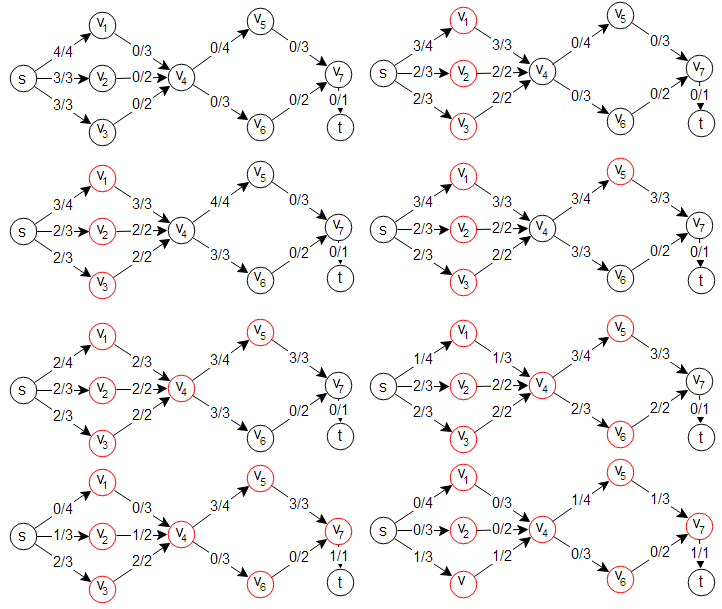
\includegraphics[width=120mm]{GRBadBlockingExample.png}
\caption{Example of multiple activations of a single node}
\label{GR-BadBlockingExample}
\end{figure}

The following table shows the order of the nodes in $L$ and the work done throughout the execution of the blocking flow algorithm on the example. Blocked nodes are underlined.
The images are named from a in the topmost left corner to h in the bottommost right corner. The third column show what operations have been done
to reach the next image. The first image shows how all edges outgoing from the source has been saturated.

In the table: To pull flow means to perform a pull operation in the graph. Pushing flow is the same as performing a push operation. Sending flow is doing a send operation.
Linking is doing a link operation.

\makebox[\textwidth][c]{
\begin{tabular}{ l | c | p{7cm}}
\hline
image & order of $L$ & Operations done \\
\hline
  a & $v_1v_2v_3v_4v_5v_6v_7$ & 
  Node $v_1$ pushes 3 flow to $v_4$, blocks itself and pulls 1 flow back to the source.
  
  Node $v_2$ and $v_3$ both pushes 2 flow to $v_4$, blocks them self and pulls 1 flow back to the source \\
  \hline
  b & $\underline{v_1v_2v_3}v_4v_5v_6v_7$ & 
 Node $v_4$ pushes 4 saturates its outgoing edges and becomes inactive\\
  \hline
  c & $\underline{v_1v_2v_3}v_4v_5v_6v_7$ & $v_5$ saturates its edge, blocks itself and pulls 1 flow back to $v_4$\\
  \hline
  d & $\underline{v_5v_1v_2v_3}v_4v_6v_7$ & $v_4$ is blocked and pulls one flow to $v_1$, $v_1$ sends it to the source\\
  \hline
  e & $\underline{v_4v_5v_1v_2v_3}v_6v_7$ & $v_6$ saturates its edge, is then blocked and pulls one flow to $v_4$ which in turn sends it to the source\\
  \hline
  f & $\underline{v_6v_4v_5v_1v_2v_3}v_7$ & $v_7$ saturates its outgoing edge, blocks itself and pulls two flow to $v_6$. $v_6$ sends this flow to the source,
  but this means that $v_4$ get active to cut it dynamic tree edge to $v_1$ as there is not capacity on it do pull two units of flow. $v_4$ links to $v_2$
  and sends the remaining one flow to the source.\\
  \hline
  g & $\underline{v_7v_6v_4v_5v_1v_2v_3}$ & $v_7$ continues by pulling two units of flow to $v_5$. This is again sent to the source. $v_4$ becomes active again
  as it saturates its pull edge in the dynamic tree. $v_4$ end up linking itself to $v_3$ to pull the last one unit of flow to the source.\\
\hline
\end{tabular}
}\\\\

In between f and g node $v_7$ is blocked. No further nodes are blocked in the rest of the run of the algorithm, yet node $v_4$ is activated twice afterwards. Twice
$v_4$ has to cut its edge in the dynamic trees and set up a new one. This breaks the theory of a node only being activated once in-between nodes being blocked.
This example does not appear that bad, as we only have a factor increase in activations. It is possible to construct a even worse example with $O(n^3)$
activation using $O(n^2)$ edges. This means that the running time bound is broken even if we spend only constant amount of time on each activation, which we do not. 

What is the actual issue that breaks the theory? It appears as if the action of moving blocked nodes to the front of the list $L$ should
make sure that flow having reached a dead end is moved back into nodes which can potentially use it before the algorithm continues.
The intuition is that if a flow has been moved through a series of nodes and get stuck, then simply reverse the direction of the
flow and push it back until it can move in a new direction. The way to do this would be to put the blocked nodes in a reverse
order in $L$, compared to the order they had in an unblocked state. Since the graph is a layered graph, the order in each layer does not matter,
only the order in which the different layers appear should be reversed. 
The example graph shows that the blocked nodes foremost in $L$ is not always in a reversed order layer-wise. Notice how the layer containing node $v_6$ and $v_5$
is split by the layer containing $v_4$. If the order had been corrected both $v_6$ and $v_5$ would have been processed before $v_4$ when doing the pulling and 
$v_4$ would only have been activated once in between node being blocked. We therefore propose an addition to $L$ to make it work.

Our idea is to add another linked-list $L_R$ of sub-lists. This list initially contains all the nodes in a reverse topological sorted order,
meaning the reverse order of $L$. If a node is blocked we remove it from $L$ and instead manipulates the corresponding node in $L_R$ in the future.
Before a node gets blocked its corresponding node in $L_R$ is not touched.
When getting the first active node, the algorithm should then look into $L_R$, and only if no active nodes exist here should it look into $L$.
Adding this new list means that the nodes in $L$ and $L_R$ never has to change order. All in all this gives a new selection behaviour that
is quite like the old one, now just with a perfect reverse ordering in front of $L$ in the form of $L_R$.

Each graph node is giving a link to its corresponding node in $L$ and $L_R$. The nodes in $L$ and $L_R$ has a similar link in 
the opposite direction to the graph node they represent.
In this way we can with $O(1)$ overhead manipulate the correct nodes by determining whether a node should be manipulated in $L$ or $L_R$. 
This is done by following the links and checking if the graph node is blocked.

The Finger tree data structure has the following amortized time operations:
\begin{description}
	\item[Initialize($V$)] \hfill \\
	Initializes a Finger tree with $|V|$ nodes. It takes $O(n\log{n})$ time.
	\item[Head($$)] \hfill \\
	Access first element, the Head, of a Finger Tree. Takes $O(1)$ time.
	\item[Split($v$)] \hfill \\
	Given a node $v$ in a Finger tree split the Finger tree in two trees $l_1$ and $l_2$. $l_1$ contains all the nodes before $v$ and $l_2$ the rest. 
	Takes $O(1+\log{(\min{l_1}{l_2})})$ time.
	\item[Concatenate($l_1,l_2$)] \hfill \\
	Concatenate the two Finger trees $l_1$ and $l_2$. Takes $O(1+\log{(\min{l_1}{l_2})})$ time.
\end{description}

The later proofs of the running time requires the split operation to take constant time. To facilitate this we would like to prove that the
concatenation operations can pay for the extra work done by the splits. 

\begin{lemma}
	The way the blocking flow algorithm uses the Finger trees, allows the amortized time of the split operation to be $O(1)$
\end{lemma}
\begin{proof}
The argument uses a potential method $\Phi = \sum_{i=0}^{k}{-1-\log{|l_i|}}$ where $l_0,\dots,l_k$ are all the sub-list, represented as Finger trees, in
$L$ and $L_R$. 
The potential starts out as zero and ends at a negative of at most $-2 - 2\log{n}$ in the end of the algorithm, where $L_R$ only consist
of a single sub-list containing all elements, and $L$ similarly is only a single sub-list containing all elements, except the ones having been removed due to block operations.

This means we end up owing up to $-2 - 2\log{n}$ at the end of the algorithm. Paying this $O(\log{n})$ cost does not break the cost of algorithm. 

The initialization leads to an increase of $-2\log{n}$, which does not change the cost of the operation.

The access operation does not change the potential at all.

A split leads to a change in potential of:
\begin{align*}
	\Phi_{after} - \Phi_{before} & = (-1 - \log{l_1} - 1 - \log{l_2}) - (-1 - \log{l_1+l_2})\\
	& \leq (-1 - \log{l_1} - \log{l_2} + 1 + \log{\max{l_1,l_2}})\\
	& = - \log{\min{l_1,l_2}}
\end{align*}
A fact used here is that $\log{a+b} \leq \log{2\max{(a,b)}} = 1 + \log{\max{a,b}}$.
This leads to a new running time of the split operation: 
\begin{align*}
	\text{Amortized time} & = \text{Actual-Time} + \text{Change in potential}\\
	& \leq (1+\log{(\min{l_1,l_2})}) - \log{(\min{l_1,l_2})}\\
	& = O(1)
\end{align*}
Similarly the new cost of the concatenations becomes  
\begin{align*}
	\Phi_{after} - \Phi_{before} & = (-1 - \log{l_1+l_2}) - (-1 - \log{l_1} - 1 - \log{l_2})\\
	& \leq (1 - \log{\max{l_1,l_2}} + \log{l_1} + \log{l_2})\\
	& = (1 + \log{\min{l_1,l_2}})
\end{align*}
Adding this additional increase of potential to the running time, gives a new amortized running time of
\begin{align*}
	\text{Amortized time} & = \text{Actual-Time} + \text{Change in potential}\\
	& \leq (1+\log{(\min{l_1,l_2})}) + (1 + \log{\min{l_1,l_2}})\\
	& = O(1+\log{(\min{l_1,l_2})})
\end{align*} $\square$
\end{proof}

The following proof gives a bound on the time spent maintaining $L$ and $L_r$, and also selecting which nodes to discharge.
\begin{lemma}
	Using Finger trees to represent the sub-lists in $L$ and $L_r$ leads to a maintaining time of $O((m+\frac{n^2}{k})\log{k})$. 
	The time spent selecting the nodes to discharge is also included in this bound.
\end{lemma}
\begin{proof}
	
	To initialize the lists the nodes are fist sorted in topological order. This takes $O(m+n)$ time. Then $L$ is initialized
	with the nodes in this order, taking $O(n\log{n})$ time. Finally $L_R$ is similarly initialized with all the nodes,
	though in the reverse order of $L$, also taking $O(n\log{n})$ time.
	
	According to lemma~\ref{BF-NodeActivations} the number of node activations is $O(m+\frac{n^2}{k})$. Each active node
	has to be discharged once. to discharge a node the algorithm only has to look at the head of the two first sub-list
	in both $L$ and $L_R$. This takes constant time. Leading to a bound on selecting nodes in the discharge operation of
	$O(m+\frac{n^2}{k})$.
	
	Each node activation leads to a split, each split takes amortized constant time according to the previous lemma.
	The time spent splitting sub-lists whenever a node gets activated is thus $O(m+\frac{n^2}{k})$. 
	
	When a nodes gets blocked it is removed in $L$ and activated in $L_R$. To remove a node $v$ in $L$ we first split
	the sub-list starting right after $v$. Since $v$ has to be active to be blocked it has to be the head of its sub-list,
	therefore one of the sub-lists after the split only contains $v$. This sub-list containing only $v$ is deleted after the split. 
	Finally the remainder of the old sub-list is concatenated to the predecessor sub-list in $L$. The node corresponding to $v$ is then 
	activated in $L_R$ leading to a split. A block operation therefore leads to two splits and a single concatenation being performed.
	The splits takes constant time, the concatenation at most $O(\log{n})$. Only $O(n)$ block operations happen leading to a combined time
	of $O(n\log{n})$.
	
	The last thing to bound is the number of concatenation happening due to a discharge operation making a node inactive. 
	Let us look at an interval between two block operation and bound how much work is done concatenating the sub-lists.
	When doing a discharge operation on node $v$ this leads to the sub-list containing $v$, denoted $S(v)$, to be
	concatenated with its preceding list, if such a list exist. Since the discharge treats all the nodes in a left to right manner, 
	each successive concatenated sub-list $S(v),S(w),\dots$ is vertex-disjoint. 
	
	We denote a sub-list \emph{small} if it contains at most $k$ elements and \emph{large} otherwise. 
	
	Each small sub-list takes $O(\log{k})$ time to concatenate. Since each active node has to be discharged, the number of small sub-lists could
	be equal to the number of node activations leading to the time spent on the small lists to also be $O((m+\frac{n^2}{k})\log{k})$.
	
	The number of large sub-lists is $l \leq \frac{2n}{k}$. Denote the large sub-lists $S_1,S_2,\dots,S_l$. The time spent to concatenate
	them in a single interval is:
\begin{align*}
	\text{Time to concatenate} & = \sum_{i=1}^{l}{\log{(1+|S_i|)}}\\
	& \leq l \log{(1 + \frac{2n}{l})} \\
	& \leq \frac{2n}{k} \log{(1 + k)}
\end{align*}
	The first inequality is because the worst case situation occurs when all the sub-list have an equal size.
	Summing over all $O(n)$ intervals in-between nodes being blocked gives a bound of $O(\frac{n^2}{k}\log{k})$ time
	spent on the large sub-lists.
	
	Adding all the different contributions together gives the bound in the lemma of $O((m+\frac{n^2}{k})\log{k})$. 
	We removed the $n\log{n}$ term since it is dominated by the rest of the expression as $k$ has to be equal or larger than two. $\square$
\end{proof}
	
This means our contribution has the exact same bound as the original theory. 

\subsubsection{Implementation modifications}\label{BF90-ImplementationModifications}
The above sections described the blocking flow algorithm as it was described in the paper \cite{GoldbergTarjan1990}. 
We have had to make some modifications to make it work in our scenario, where we work on a graph of super-nodes.

The blocking flow algorithm only work on DAGs, but since we do not remove any edges, the input graph does not have to be a DAG.
What we really want is to only use the edges that are admissible. The definition from admissible comes from the Goldberg And Rao maximum flow algorithm.
We therefore adds the same length computation to the blocking flow, so that we can distinguish which edges to use and which not to use.
On last thing we need to check is that we do not make any push or pull operations between sub-nodes of the same super-node. This is
easily done by following the super-node pointers of the two operands and check whether they are equal.

In many of the maximum flow algorithms we store the flow by manipulating the residual graph to save space. In the blocking flow algorithm we actually store
the flow values explicitly on the edges, as the maximum flow algorithm needs to manipulate these values before they are used to augment the flow in the graph.

The biggest change compared to the theory is that we do not user Finger-trees to represent the sub-lists in $L$. Instead we have chosen to 
replace $L$ by a first-in-first-out queue similarly to the Goldberg and Tarjan 1988 push relabel algorithm. This was done to make the implementation simpler.
The cost however is a big change in the running time. The change comes from an increase in node-activations, the following lemma gives a bound:
\begin{lemma}
	The number of node-activations using a FIFO queue is $O(n^2 + \frac{n^3}{k})$
\end{lemma}
\begin{proof}
	Connect all the nodes with the edges the can transfer flow on called this graph $G_f$. 
	In case of unblocked nodes this will be the edges that they can push on,
	for blocked nodes it is the edges they can pull on. A node is only able to activate those it is connected to. 
	No cycles can appear in $G_f$. This is the case as that would mean a cycle in the labels, which can not happen as the admissible edges create a DAG.
	Another case creating cycles in $G_f$ would be if an edge can both be pushed and pulled on at the same time, but that can not be the case.
	
	The scenario giving the most node activations is if $G_f$ is one long line of nodes $v_0,v_1,\dots,v_n$. Where $v_0$ is the source or target.
	Node $v_i$ can transfer excess to $v_{i-1}$, meaning they are connected and that $v_i$ can activate $v_{i-1}$. Assume the worst, that all nodes, besides
	the source and target, are active. Then the worst order to pick the nodes in would be to follow this simple procedure:
	Process the node with the lowest index $i$ by transferring all it excess flow into node $v_{i-1}$, reiterate until no nodes are active.
	This would lead to a worst case behaviour where $v_1$ would be made inactive by transferring its flow to $v_0$, 
	then $v_2$ would transfer all its flow to $v_1$ activating it again, $v_1$ would then be made inactive by it transfering its flow to $v_0$, $v_3$ would then be processed activating 
	$v_2$, which in turn activates $v_1$ etc.
	This would lead to the number of activations being $1+2+3+\dots+n = O(n^2)$. 
	
	The dynamic tree data structure saves this a little. If a node
	is processed it would link itself in the dynamic tree to its predecessor in $G_f$ making the transfer of flow cheaper next time it would be activated.
	If the entire path is in dynamic trees then the number of nodes being activated for a node with index $i$ would be $\frac{i}{k}$ as each dynamic
	tree has a maximum size of $k$, so each time $k$ nodes has been passed, a new dynamic tree is used, costing a node-activation. This would mean
	the new bound is $(1+\frac{1}{k})+(1+\frac{2}{k})+(1+\frac{3}{k})+\dots+(1+\frac{n}{k}) = O(n + \frac{1}{k}(1+2+3\dots+n)) = O(n + \frac{n^2}{k})$. 
	The constant term each paying for first time a node is processed, where it does its link operation. 
	
	Every time we block a node we could change $G_f$. This means that all these activations could happen again in each interval between a block.
	Since there is $O(n)$ intervals in-between nodes being blocked the number of node activations are $O(n + \frac{n^2}{k}) \cdot O(n) = O(n^2 + \frac{n^3}{k})$
	$\square$
\end{proof}
This is an increase compared to the previous bound of $O(m + \frac{n^2}{k})$. This increase propagates through the rest of the theory making the final
running time of our implementation $O((n^2+\frac{n^3}{k})\log{k})$. Still setting $k$ equal to $\frac{n^2}{m}$, leads to a bound of
$O\left((n^2 + nm)\log{\frac{n^2}{m}}\right)$. 

Since we no longer need a topological sorting to make $L$ initially, we have removed it.

\subsection{Haeupler And Tarjan Routing Algorithm}\label{GR-RF}
We use a routing flow algorithm made by B. Haeupler and R. E. Tarjan, it was published in 2007, \cite{Haeupler2007}.
Using this algorithm instead of the original one leads to a constant decrease in running time of the maximum flow algorithm.
The two routing flow algorithms have the same theoretical running time.

When the blocking flow algorithm has been run some sub-nodes in each super-node can have flow going into them or out of them.
We can calculate these values. We denote all flow going into a node as \emph{supply} and everything going out as \emph{demand}.
Every super-node, besides the ones containing the source and the target, has to have equal supply and demand when summed over
all the sub-nodes in super-node. The super-node containing the source has a higher demand than supply, and the super-node
containing the target is the opposite way.

Since each super-nodes is a strongly connected component, it is possible for each SCC to pick a node $v$ and build an in-tree and an out-tree with $v$ as its root.
The in-tree is a tree where every node in the tree can reach the root. The out-tree is a tree where the root can reach every node in the tree.
The idea is then to route all the supply via the in-tree to the root, and all the demand via the out-tree to the root as well.
The pseducode for the main idea of the algorithm can be seen in Algorithm~\ref{RFAlg}

\begin{algorithm}
\caption{Routing Flow - algorithm}\label{RFAlg}
\begin{algorithmic}[1]
	\Statex
\Require A list $L$ of Strongly Connected Components $\in {G(V,E)}$ and a way \Call{SameSCC}{$v,w$} of knowing if 2 nodes are in the same component.
\Procedure{RouteFlow}{}
	\ForAll{$v \in V$}
		\State Calculate supply and demand for $v$
	\EndFor
	\ForAll{Strongly-Connected-Components $\in L$}
		\State\State choose a node $v$ to be the root
		\State\Call{BuildInTree}{$v$}
		\State\Call{BuildOutTree}{$v$}
		\State\Call{RouteFlow}{$v$}
	\EndFor
\EndProcedure
\Statex
\Procedure{BuildInTree}{$v$}
	\State $Q \gets Queue$
	\State Add $v$ to the rear of $Q$
	\While{{$Q \neq \emptyset$}}
		\State Node $w \gets$ first element of Q, removed from the queue.
		\ForAll{$\{(u,w)\mid \Call{SameSCC}{$u,w$}$ and $\Call{IsZeroEdge}{(u,w)}\}$}
			\If{$u.InTreeParent = nil$}
				\State $u.InTreeParent \gets w$
				\State Add $u$ as a child of $w$ in the InTree
				\State Add $u$ to the rear of $Q$
			\EndIf
		\EndFor
	\EndWhile
\EndProcedure
\end{algorithmic}
\end{algorithm}
The pseudocode in Algorithm~\ref{RFAlg} also shows how to build an in-tree. A queue is used to keep track of all the nodes that should be processed.
When a node is processed it looks at all its incoming edges. If an edge $(u,w)$ goes between nodes in the same SCC and is a zero-length edge it could be that
the edge should be part of the in-tree. It should only be part of the tree if $u$ has not been processed before. We can check this by seeing if it has a
parent assigned in the tree. If that is not the case then we add $w$ as $u$'s parent and add $u$ to the queue. 

To start the construction any node $v$ is selected from the SCC and appointed as the root. 

An out-tree is constructed in a similar way, the edges considered are the outgoing edges instead of the incoming ones.

When constructing the in- and out-tree for the SCC containing the source and the target, the source and target nodes are always selected to be the root of the trees.

The rest of the algorithm consists of three DFS's of the trees constructed.

First we do a DFS run of the out-tree where we calculate a value called the \emph{descendant demand}, 
it is the sum of all the demands of the children plus the node itself.

We then do a DFS run in the in-tree where we process the nodes bottom-up. The idea is to route the supply to the root.
When we process a node $v$ with parent $w$ we calculate the amount of supply to move. The supply moved, $sm$, is set to 
the minimum of $v$'s supply and $\Delta$ minus the descendant demand of $v$. The flow on edge $(v,w)$ is increased by $sm$,
the supply of $v$ is decreased by $sm$ and the supply of $w$ is increased by the same amount. The idea is that
we only move extra flow and excess closer to the root if we know that another part of the sub-tree of $v$ does not have
a demand for it.

The last thing done is a DFS run in the out-tree where the demand is moved towards the root. When a node $v$ with parent $w$
is processed we move an amount corresponding to the difference in demand and supply closer to the root in a
similar fashion as in the previous DFS run.

The pseudocode for the three DFS runs can be seen in Algorithm~\ref{RFAlg-cont}.

\begin{algorithm}
\caption{Routing Flow - algorithm(cont.)}\label{RFAlg-cont}
\begin{algorithmic}[1]
\Statex
\Procedure{RouteFlow}{$v$}
	\State\Call{CalculateDescendantDemandsRecursively}{v}
	\State\Call{MoveSupplyForwardRecursively}{v}
	\State\Call{MoveDemandBackwardRecursively}{v}
\EndProcedure
\Statex
\Function{CalculateDescendantDemandsRecursively}{$v$}
	\State $v.dd \gets v.demand$
	\ForAll{$w \in OutTreeChildren(v)$}
		\State $v.dd \gets v.dd + \Call{CalculateDescendantDemandsRecursively}{w}$
	\EndFor
\EndFunction
\Statex
\Procedure{MoveSupplyForwardRecursively}{$v$}
	\ForAll{$w \in InTreeChildren(v)$}
		\State $\Call{MoveSupplyForwardRecursively}{w}$
	\EndFor
	\State $supplyToMove \gets \min{(v.supply, \Delta - v.dd)}$
	\State $v.supply \gets v.supply - supplyToMove$
	\State $(v,w) \gets v.InTreeParentEdge$
	\State $f(v,w) \gets f(v,w) + supplyToMove$
	\State $w.supply \gets w.supply + supplyToMove$
\EndProcedure
\Statex
\Procedure{MoveDemandBackwardRecursively}{$v$}
	\ForAll{$w \in OutTreeChildren(v)$}
		\State $\Call{MoveDemandBackwardRecursively}{w}$
	\EndFor
	\State $demandToMove \gets v.demand - v.supply$
	\State $(w,v) \gets v.OutTreeParentEdge$
	\State $f(w,v) \gets f(w,v) + demandToMove$
	\State $w.demand \gets w.demand + demandToMove$
\EndProcedure
\end{algorithmic}
\end{algorithm}
The original algorithm just routed the entire supply and demand to the root. This could lead to the flow of an edge being $2\Delta$, 
$\Delta$ flow being used on the supply and $\Delta$ flow on the demand. Since they also needed $\Delta$ slack for the special edges
the original length function had to have non-special zero-length edges have a capacity greater or equal to $3\Delta$. Since this new
algorithm accounts for demand being used in the sub-trees it never routes both supply and demand to the root, thereby saving
up to $\Delta$ amount of flow on each edge, leading to the distance function we have used.

Building the in- and out-tree takes $O(m)$ time. Each node is only processed once. The work done when processing a node is having its edge-list run
through once plus some constant time work. This sums up to $O(m)$ over all nodes.

The DFS's all takes $O(n)$ time. The total running time of the routing algorithm is therefore $O(m+n) = O(m)$

\subsubsection{Implementation modifications}
This algorithm uses recursion. This gives us some trouble as the recursion stacks ends up taking to much memory, crashing the algorithm in 
instances with large strongly connected components. 
We therefore rewrote the code to use just an array as our own version of a stack.
When we visit a child in the DFS we put a pointer to the parent node on the first empty entry in the array, then we can easily go back to the 
parent when done processing the child. Since each root to node path can be at most $n$ we only use an array of this size.
The extra book-keeping time is constant, so the running time is the same. Since we use the same array all the time, we pre-allocate it
and use it in all iterations.